\documentclass{article}
\usepackage{style-notes}

\newcounter{lecnum} 	% define counter for lecture number
\renewcommand{\thepage}{\thelecnum-\arabic{page}}	% define how page number is displayed (< lecture number > - < page number >)
% define lecture header and page numbers
% NOTE: to call use \lecture{< Lecture # >, < Lecture name >, < Chapter # >, < Chapter name >, < Section #s >}
\newcommand{\lecture}[5]{

    % define headers for first page
    \thispagestyle{empty} % removes page number from page where call is made

    \setcounter{lecnum}{#1}		% set lecture counter to argument specified

    % define header box
    \begin{center}
    \framebox{
      \vbox{\vspace{2mm}
    \hbox to 6.28in {\textbf{MATH 320: Probability} \hfill}
       \vspace{4mm}
       \hbox to 6.28in {{\hfill \Large{Lecture #1: #2} \hfill}}
       \vspace{2mm}
       \hbox to 6.28in {\hfill Chapter #3: #4 \small{(#5)}}
      \vspace{2mm}}
    }
    \end{center}
    \vspace{4mm}
    
    % define headers for subsequent pages
    \fancyhead[LE]{\textit{#2} \hfill \thepage} 		% set left header for even pages
    \fancyhead[RO]{\hfill \thepage}		% set right header for odd pages

}

% define macros (/shortcuts)
\newcommand{\bu}[1]{\textbf{\ul{#1}}}			% shortcut bold and underline text in one command
\newcommand{\blankul}[1]{\rule[-1.5mm]{#1}{0.15mm}}	% shortcut for blank underline, where the only option needed to specify is length (# and units (cm or mm, etc.)))
\newcommand{\comp}[1]{{\sim}#1}		% shortcut for complement of event ~A (tilde without extra space)


% NOTES on what didn't cover
% Theory lecture 2 -> counting unordered with replacement


\begin{document}

\lecture{2}{Counting}{1}{Probability}{1.2}

\bu{Counting basics}\bigskip

Motivation
\begin{itemize}
    \item There are ways to count the number of outcomes in certain types of random experiments. Thus, we need to develop some counting principles.
    \item[] This is useful in finding probabilities of events associated with these random experiments.
    \item Example: Suppose we have a shuffled deck and we deal seven cards. What is the probability that we draw no queens?
\end{itemize}\vspace{40pt}

Simple counting examples
\begin{enumerate}
    \item Suppose our class 100 students. 78 students are mathematical science majors and 50 students are actuarial science majors. 41 students are double majors in mathematical science and actuarial science.
    \begin{enumerate}
        \item How many students are not mathematical science majors?\vspace{20pt}
        \item How many students major in mathematical sciences or actuarial sciences?\vspace{20pt}
    \end{enumerate}
    \item A single card is drawn from a well-shuffled deck. How many cards are hearts or clubs?
\end{enumerate}\vspace{20pt}

Venn diagrams\bigskip
\begin{itemize}
    \item \textbf{Venn Diagrams} are helpful for visualizing all of the components of a counting problem and can easily extended to three events.    
\end{itemize}\vspace{80pt}

Basic rules\bigskip
\begin{itemize}
    \item \textbf{Notation}: The number of elements in the event (set) $A$ = \\
    \item \textbf{Complements counting rule}: For any finite sample space $S$ and event $A$ \\
    \item \textbf{General union counting rule}:
    \item[] For any two events $A$ and $B$ in any finite sample space \\
    \item \textbf{Special case union counting rule}: If $A$ and $B$ are mutually exclusive\bigskip
\end{itemize}\bigskip

Counting outcomes of an experiment\bigskip
\begin{itemize}
    \item \textbf{Tree diagrams} give a simple graphical display of all possible cases (pairs of outcomes) in problem/experiments if the number of outcomes is not unreasonably large.
     \item[] When drawing tree diagrams, think about the stages of the experiment.\bigskip
    \item Example: Suppose we are testing for the presence of a disease. There are two things two consider, if the person has the disease (which is unknown) and the result of the test, positive or negative. Let's define:
    \begin{flalign*}
       D &= \text{the person tested has the disease}&\\
       \comp D &= \text{the person tested does not have the disease}&\\
        Y &= \text{the test is positive}&\\
        N &= \text{the test is negative}&
    \end{flalign*}
    \item[] Find how many outcomes are possible and what each of them are.\vspace{200pt}
    \item When experiments get larger, we can use the following idea.\bigskip
    \item \textbf{Multiplication principle for counting}:
    \item[] If a job consists of $k$ separate tasks, the $i$th of which can be done in $n_i$ ways \\ ($i = 1, \ldots, k$), then the entire job can be done in $n_1 \times n_2 \times \cdots \times n_k$ ways.\bigskip\\
    \begin{tabular}{| c | c | c | c || c |}
        \hline
        Task 1 & Task 2 & $\cdots$ & Task $k$ & Total outcomes\\
        \specialrule{.1em}{.05em}{.05em}
        $n_1$ & $n_2$ & $\cdots$ & $n_k$ & $n_1 \times n_2 \times \cdots \times n_k$\\
        \hline
    \end{tabular}\bigskip
    \item Example: Sally has 6 pairs of socks, 4 shorts, 5 shirts, and 3 sunglasses. How many ways can she get dressed?\vspace{15pt}\\
    \item It is very important to correctly define the sub experiments, then can just use the rule. Each``task / sub experiment'' is like a level in our tree diagram.
    \item[] This is also an important principle because we can use it to develop some more counting techniques.
\end{itemize}\bigskip

\bu{Permutations, combinations and partitions}\bigskip

Counting number of ways\bigskip
\begin{itemize}
    \item After defining tasks in an experiment, often we need to count the number of possible ways to perform each task. In doing so, there are four important criteria to consider:
    \begin{enumerate}
        \item The number of distinguishable items
        \item The number of objects we are going to select
        \item Order matters or not?
        \item With replacement or without?
    \end{enumerate}\bigskip
    \item Possible methods of counting\\
    \begin{figure}[H]
        \center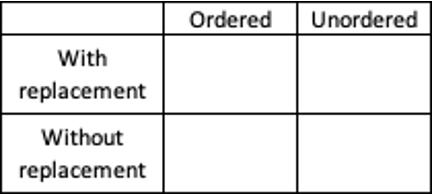
\includegraphics[scale=0.75]{test-1/counting-table}
    \end{figure}
\end{itemize}

\newpage

Ordered, with replacement\bigskip
\begin{itemize}
    \item Example: How many four-letter words can the letters A through Z produce?\vspace{30pt}
    \item \textbf{Ordered, with replacement}: Given $n$ distinguishable objects, there are \blankul{1cm} ways to choose with replacement an ordered sample of $r$ objects.\bigskip
    \item \textit{STRATEGY}: When doing counting problems, think about (and actually draw) the ``slots''. This will help with what numbers to use AND to determine if order matters.
    \item[] This illustrates an application of the multiplication principle where each ``slot'' is a separate task.
\end{itemize}\bigskip

Ordered, without replacement\bigskip
\begin{itemize}
    \item Example: How many ways can Bob, Mary and Jane sit in three seats?
    \item[] This question is really asking how many \blankul{3cm} of these three are there?\vspace{30pt}
    \item \textbf{Ordered without replacement (all $\boldsymbol{n}$)}: The number of permutations of $n$ distinct objects is \blankul{7cm}.\bigskip\bigskip
    \item Example: What is the number of four-letter code words selecting from the 26 letters of the alphabet without replacement?\vspace{30pt}
    \item \textbf{Ordered without replacement ($\boldsymbol{r \le n}$)}: The number of $r$-permutations of $n$ distinct objects (aka \textbf{permutation} of $n$ objects taken $r$ at a time) is \blankul{2cm}.\vspace{100pt}
    \item[] Example: $P{10 \choose 3} = $
\end{itemize}

\newpage

Unordered, without replacement\bigskip
\begin{itemize}
    \item Two scenarios: Among 8 students, (a) selecting 1\textsuperscript{st}, 2\textsuperscript{nd} and 3\textsuperscript{rd} place winners \\ (b) selecting 3 committee members among 8 students. What is the difference?\vspace{30pt}
    \item \textbf{Unordered without replacement ($\boldsymbol{r \le n}$)}: The number of combinations of $n$ objects taken $r$ at a time is \blankul{4cm}.\vspace{40pt}
    \item[] A \textbf{combination} is an unordered group (more formally, an $r$-element subset of the original $n$ distinct objects), and ${n \choose r}$ counts the total number of different groups possible.\bigskip
    \item Useful property: \hspace{10pt} $\displaystyle {n \choose r} = $
    \item[] If a group of $r$ is made, then a group of $n - r$ is made and vice versa.\end{itemize}\bigskip

Relationship between combinations and permutations\bigskip
\begin{itemize}
    \item Both of these can be thought of as two sub experiments involving the other and demonstrates how \textbf{order} impacts the counting tool.\\
    \item[] Permutation $\longrightarrow$ Combination \hfill Combination $\longrightarrow$ Permutation \bigskip\\
    \begin{tabular}{l l}
        1. \hspace{215pt} & 1. \\\\
        2. \hspace{215pt} & 2. \\
    \end{tabular}\vspace{60pt}
    \item[] Example: Committee of 3 from 7 \hspace{90pt} Example: Rank 3 from 7\vspace{200pt}
\end{itemize}\bigskip

Examples\bigskip
\begin{enumerate}
   \item Determining ordered vs unordered.
   \item[] Find the number of ways to do each of the following.
    \begin{enumerate}
        \item Rank your favorite 4 desserts from the menu of 10 items.\vspace{40pt}
        \item Select which 3 side dishes to serve out of the 15 from your cookbook.\vspace{40pt}
        \item Determine the jobs for three members out of 8 at the dinner party: set the table, serve the food, do the dishes.\vspace{40pt}
    \end{enumerate}
    \begin{itemize}
        \item In some problems involving ordering, the ordering is not obvious or implied, but rather implicit (like when making an assignment list).
        \item[] BEST way to think about it: If the ``slots'' have \blankul{2cm}, then order \blankul{2cm}.
    \end{itemize}\bigskip
    \item Combined problems
    \item[] A company has 20 male employees and 30 female employees. They are forming a committee that will have two male members and three female members. In how many ways can this committee be chosen?\vspace{140pt}
    \begin{itemize}
        \item Many counting problems include combined the use of the multiplication principle, permutations and combinations.
        \item[] So just separate a scenario into tasks, count each task individually and then multiply each tasks total ways to get the total overall number of ways.
    \end{itemize}
\end{enumerate}\bigskip

More than two groups\bigskip
\begin{itemize}
    \item \textbf{Partitioning} refers to the process of breaking a large group into separate smaller groups.
    \item[] Will learn how to count number of ways to divide all available objects:
    \begin{figure}[H]
        \center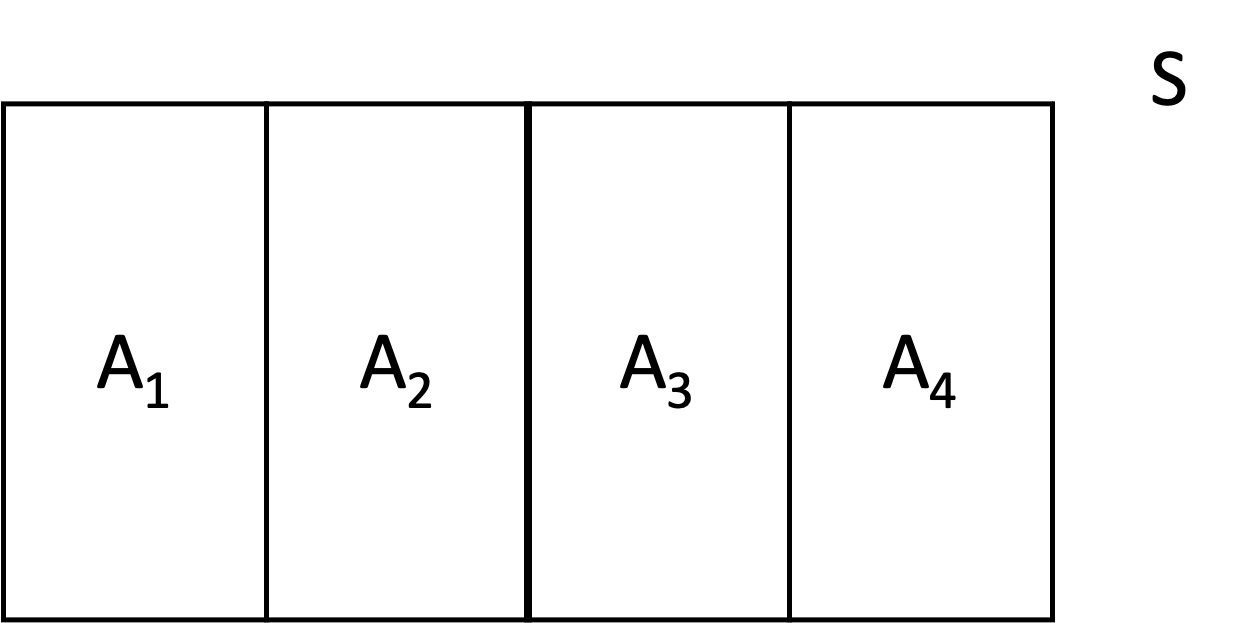
\includegraphics[scale=0.4]{test-1/partition}
    \end{figure}
    \item[] The combination problems previously discussed are simple examples of partitioning problems.
    \item Example: Flip 5 coins. How many observation sequences are there in which there are two heads and three tails?\vspace{50pt}
    \item The basic idea of a combination divides $n$ distinct objects into two groups:\\ a group of chosen objects and a group of unchosen objects.\bigskip
    \item[] This is why \hspace{10pt} $\displaystyle {n \choose r} =  {n \choose {n - r}}$\hspace{10pt} is called a \textbf{binomial coefficient}.
    \item This can be extended to more than two groups.
    \item[] Example: There are 10 students. How many ways can we make three groups with sizes 3, 3 and 4.\vspace{40pt}
    \item \textbf{Counting partitions}: The number of partitions of $n$ objects into $k$ distinct groups of sizes $n_1, n_2, \ldots, n_k$ (where $n_1 + \cdots + n_k = n$ $\Longleftrightarrow$ splitting up entire group) is given by:\bigskip\\
    $\displaystyle {n \choose {n_1,\, n_2,\, \ldots,\, n_k}} = $\vspace{20pt}
   \item[] This is called the \textbf{multinomial coefficient}.
   \newpage
   \item Example: Find the number of ways to rearrange the letters in the word MISSISSIPPI.\vspace{60pt}
   \item Counting partitions can also be thought of as the number of ways to arrange $n$ objects where $n_1$ objects are alike, $n_2$ objects are alike and so forth.
   \item[] To account for the repetitions when counting distinct permutations (arrangements), we need to \blankul{7cm}.
   \item[] It is the groups that matter, not the order within the groups.
\end{itemize}\bigskip

Summary: When to use which counting tool (formula)\bigskip
\begin{itemize}
    \item \textbf{Ordered}
    \begin{itemize}
        \item \textbf{With replacement}: \blankul{2cm} \quad ex) how many 6 digit passwords can the digits 0-9 make?
        \item \textbf{Without replacement}: \blankul{2cm} \quad ex) 7 possible vacation destinations, rank your top 3.
    \end{itemize}
    \item \textbf{Unordered}
        \begin{itemize}
        \item \textbf{Without replacement}: \blankul{2cm} \quad ex) select 5 out of 12 players to start the basketball game.
        \item[] \textbf{More than two groups}: \blankul{2cm} \quad ex) make smaller teams of size 2, 3, and 3 from 8 players.
        \item With replacement: This exists, but we won't worry about it.
    \end{itemize}
\end{itemize}



    

    
\end{document}